\documentclass[10pt,a4paper]{article}
\usepackage{amsmath,amssymb,amsthm,graphicx}
\usepackage{amsmath,amssymb,amsthm,graphicx,xcolor}
\usepackage{hyperref}
\newtheorem{theorem}{Theorem}[section]
\newtheorem{lemma}[theorem]{Lemma}
\newtheorem{corollary}[theorem]{Corollary}
\newtheorem{proposition}[theorem]{Proposition}
\newtheorem{claim}[theorem]{Claim}
\newtheorem{conjecture}[theorem]{Conjecture}
\newtheorem{fact}[theorem]{Fact}
\newtheorem{open}[theorem]{Open Problem}
\theoremstyle{definition}
\newtheorem{definition}[theorem]{Definition}
\newtheorem{construction}[theorem]{Construction}
\newtheorem{remark}[theorem]{Remark}
\newenvironment{subproof}[1][Proof]{\begin{proof}[#1]}{\end{proof}}
\newcommand{\N}{\mathbb N}
\newcommand{\R}{\mathbb R}
\newcommand{\Z}{\mathbb Z}
\newcommand{\Si}{\mathbb S}
\def\etal{{\it et~al.}}
\newcommand{\prob}{{\rm Pr}}
\newcommand{\Exp}{{\rm E}}
\newcommand{\e}{\epsilon}
\newcommand{\ext}{{\tt ext}}
\newcommand{\extF}{{f^{\tt ext}}}
\newcommand{\ev}{\nu}
\newcommand{\bitset}{\{0,1\}}
\newcommand{\xth}{{\rm th}}
\newcommand{\jj}{\alpha}
\newcommand{\jjj}{\beta}
%
\newcommand{\imu}{{\mu^{-1}}}
\newcommand{\si}{\mu}
\newcommand{\ing}{{\tt in}}
\newcommand{\md}{{\tt mid}}
\newcommand{\outg}{{\tt out}}
\newcommand{\dG}{{\vec{G}}}
\newcommand{\dV}{{\vec{V}}}
\newcommand{\dE}{{\vec{E}}}
\newcommand{\gin}{g_{\tt in}}
\newcommand{\gout}{g_{\tt out}}

%
%
\def\xsection{\section}
\def\xsubsection{\subsection}
%
%
\newcommand{\aff}{{\rm aff}}
\newcommand{\mypar}[1]{\subparagraph{{#1}}}
%
%
\newcommand{\DF}{{\tt DF}}
\newcommand{\OSE}{{\tt OSE}}
\newcommand{\ang}[1]{{\langle{#1}\rangle}}
\newcommand{\cnt}{{\tt cnt}}
\newcommand{\vc}{{\nu}}
\newcommand{\bl}{{\tt BL}}
%
\newcommand{\qc}{{\tt qc}}
\newcommand{\sac}{{\tt sc}}
%
\newcommand{\stt}{{\rm state}}
\newcommand{\rst}{{\;\mbox{\rm s.t.}\;}}
\newcommand{\floor}[1]{{\lfloor#1\rfloor}}
\newcommand{\ceil}[1]{{\lceil#1\rceil}}
\newcommand{\round}[1]{{\lfloor#1\rceil}}
\newcommand{\xor}{\oplus}
\newcommand{\eqdef}{\stackrel{\rm def}{=}}
\newcommand{\wt}{{\rm wt}}
\newcommand{\GF}{{\rm GF}}
\newcommand{\SL}{{\rm SL}}
\newcommand{\GG}{{\hat G}}
\newcommand{\AN}{{\tt AN}}
\newcommand{\xx}[1]{{x^{(#1)}}}
%
\newcommand{\kk}[2]{{k^{(#1)}_{#2}}}
%
%
\newcommand{\fits}{{\tt fit}}
\newcommand{\xxi}[1]{{x^{(#1)}_{i_{#1}}}}
\newcommand{\xxx}[2]{{x^{(#1)}_{#2}}}
\newcommand{\rnd}{\in_R}
\newcommand{\st}{{\rm st}}
\newcommand{\nd}{{\rm nd}}
\newcommand{\rd}{{\rm rd}}
\newcommand{\ov}{\overline}
\newcommand{\ovd}{{\overline\delta}}
\newcommand{\ovp}{{\overline \tau}}
\newcommand{\tp}{{\widetilde p}}
\newcommand{\Avv}{{A_{\rm vv}}}
\newcommand{\sumh}{{\odot}}
%
\newcommand{\ovS}{{\overline S}}
\newcommand{\ovs}{{\overline s}}
\newcommand{\ovr}{{\overline r}}
\newcommand{\zo}{{\zeta_\omega}}
\newcommand{\zoo}[1]{{\zeta_{\omega_{#1}}}}
\newcommand{\ozo}{{\overline\zeta_\omega}}
\newcommand{\ozoo}[1]{{\overline\zeta_{\omega_{#1}}}}
\newcommand{\zS}{{\zeta_S}}
\newcommand{\ozS}{{\overline\zeta_S}}
\newcommand{\zT}{{\zeta_T}}
\newcommand{\ozT}{{\overline\zeta_T}}
\newcommand{\zI}{{\zeta_I}}
\newcommand{\ozI}{{\overline\zeta_I}}
\newcommand{\zJ}{{\zeta_J}}
\newcommand{\ozJ}{{\overline\zeta_J}}
%
\newcommand{\dd}{{\tt d}} 
\newcommand{\bb}{{d}} 
\newcommand{\ap}{{\alpha}}
\newcommand{\ba}{{\beta}}
\newcommand{\ovap}{{\overline\ap}}
\newcommand{\PP}{{{\tt P}}}
\newcommand{\SP}{{{\tt SP}}}
\newcommand{\papd}{{{\tt P}'_\ovap}}
\newcommand{\papdd}[1]{{{\tt P}^{({#1})}_\ovap}}
\newcommand{\papx}{{{\tt P}}}
%
%
%
\newcommand{\ee}{\chi}
%
\newcommand{\da}{\delta}
\newcommand{\SD}{\bigtriangledown}
\newcommand{\PiH}[1]{\Pi^{\rm H}_{#1}}
\newcommand{\PiE}[1]{\Pi^{\rm E}_{#1}}
\newcommand{\Pil}{\Pi^{\tt ls}}
\newcommand{\Pie}{\Pi^{\tt eq}}
\newcommand{\Pim}{\Pi^{\tt mr}}
%
\newtheorem{thm}{Theorem}[section]      
%
\newcommand{\BT}{\begin{theorem}}   \newcommand{\ET}{\end{theorem}}
\newtheorem{dfn}[theorem]{Definition}      
\newcommand{\BD}{\begin{definition}}   \newcommand{\ED}{\end{definition}}
\newtheorem{const}[theorem]{Construction}      
\newcommand{\BCT}{\begin{construction}} \newcommand{\ECT}{\end{construction}}
\newtheorem{corr}[theorem]{Corollary}      
%
\newcommand{\BCR}{\begin{corollary}} \newcommand{\ECR}{\end{corollary}}
\newtheorem{conj}[theorem]{Conjecture}      
\newcommand{\BCJ}{\begin{conj}} \newcommand{\ECJ}{\end{conj}}
\newtheorem{prop}[theorem]{Proposition}
\newcommand{\BP}{\begin{proposition}}   \newcommand{\EP}{\end{proposition}}
\newtheorem{rem}[theorem]{Remark}
\newcommand{\BR}{\begin{remark}}   \newcommand{\ER}{\end{remark}}
%
\newcommand{\BO}{\begin{open}}   \newcommand{\EO}{\end{open}}
%
%
%
%
%
\newtheorem{lem}[thm]{Lemma}  
\newcommand{\BL}{\begin{lemma}}   \newcommand{\EL}{\end{lemma}}
\newtheorem{tech-lem}{Lemma}[thm]  
\newtheorem{clm}[thm]{Claim}            
%
\newcommand{\BCM}{\begin{claim}}   \newcommand{\ECM}{\end{claim}}
%
\newtheorem{techclm}{Claim}[subsection]        
\newcommand{\Bcm}{\begin{techclm}}   \newcommand{\Ecm}{\end{techclm}}
\newtheorem{tech-obs}{Observation}[theorem]          
\newcommand{\Bobs}{\begin{tech-obs}}   \newcommand{\Eobs}{\end{tech-obs}}
%
%
%
\newtheorem{tech-def}[tech-lem]{Definition}            
%
\newtheorem{tech-const}{Construction}[subsection]     
\newcommand{\Bct}{\begin{tech-const}} \newcommand{\Ect}{\end{tech-const}}
%
\newcommand{\BE}{\begin{enumerate}}
\newcommand{\EE}{\end{enumerate}}
\newcommand{\BI}{\begin{itemize}}
\newcommand{\EI}{\end{itemize}}
\newcommand{\BDes}{\begin{description}}
\newcommand{\EDes}{\end{description}}
\def\blkslug{\hbox{\hskip 1pt\vrule width 8pt height 8pt depth 1.5pt\hskip 1pt}}
%
%
\def\FullBox{\hbox{\vrule width 6pt height 6pt depth 0pt}}
\def\qqed{$\FullBox$}
%
\newcommand{\eqrefs}[2]{{\rm Eq.~(\ref{#1})\&(\ref{#2})}}
\newcommand{\secref}[1]{Section~\ref{#1}}

%
%
\newenvironment{proofsk}{\noindent{\bf Proof Sketch:~}}{\qed}
\newcommand{\BPF}{\begin{proof}} \newcommand{\EPF}{\end{proof}}
%
\newcommand{\BPFS}{\begin{proof}[Proof Sketch]} \newcommand{\EPFS}{\end{proof}}
%
\newcommand{\Bpf}{\begin{subproof}} \newcommand{\Epf}{\end{subproof}}


\newcommand{\tildeO}{{\widetilde{O}}}
\newcommand{\tildeOM}{{\widetilde{\Omega}}}
\newcommand{\tildeT}{{\widetilde{\Theta}}}
\newcommand{\tildef}{{\widetilde{f}}}
\def\L{{\tt LOC}}
\newcommand{\dist}{{\rm dist}}
\newcommand{\LL}[1]{{\zeta_{#1}}}
\newcommand{\E}{{\tt ENV}}
\newcommand{\Ed}{{\tt ENV}^{\dagger}}
\newcommand{\Edd}{{\tt ENV}^{\ddagger}}
\newcommand{\Er}{{\tt ENV}^{(r)}}
\newcommand{\iEr}[1]{{\tt ENV}^{(r)}_{#1}}
\newcommand{\SPD}{{\Delta}}
%
\newcommand{\Right}{{\sc right}}
\newcommand{\Left}{{\sc left}}
\newcommand{\Still}{{\sc still}}
\newcommand{\Empty}{{\sc empty}}
\newcommand{\teps}{{\tilde{\eps}}}
%
%
\newcommand{\wEr}{\widetilde{\tt ENV}^{(r)}}
\newcommand{\iwEr}[1]{\widetilde{\tt ENV}^{(r)}_{#1}}
%
%

%
%
%
%
%
%
%
%
%
%
%
%
%
%
%
%
%
%
%
%
%
%
%
%
%
%
%
%
\newcommand{\IS}{{\cal IS}}
\newcommand{\DHAM}{{\cal DH}}
\newcommand{\HAM}{{\cal H}}
\newcommand{\calP}{{\cal P}}
\newcommand{\CG}{{\cal C}}
\newcommand{\CC}{{\tt CC}^{(t)}}
\newcommand{\CCC}{{\tt CC}^{(3)}}
\newcommand{\CCx}{{\tt CC}^{(t-2)}}
\newcommand{\PT}{{\tt Q}}
\newcommand{\owCC}{{\vec{\tt CC}}}
\newcommand{\simCC}{{\ddot{\tt CC}}}
\newcommand{\naPT}[1]{{{\tt Q}^{\rm na}_{#1}}}
\newcommand{\DISJkn}{{{\rm DISJ}_n^{(k)}}}
%
\newcommand{\vol}{{\rm vol}}
\newcommand{\ex}{{\rm E}}
\newcommand{\poly}{{\rm poly}}
\newcommand{\union}{{\cup}}
\newcommand{\NP}{{\cal NP}}
\renewcommand{\P}{{\cal P}}
\newcommand{\dns}{{\rho}}
%
\newcommand{\dpf}{{\varrho}}
%
\newcommand{\C}{{\cal C}}
\newcommand{\B}{{\cal B}}
\newcommand{\D}{{\cal D}}
\newcommand{\F}{{\cal F}}
\newcommand{\G}{{\cal G}}
\newcommand{\Rk}{{{\cal R}^{(k)}}}
\newcommand{\RSk}{{{\cal R}^{({\tt S},{\tt k})}}}
\newcommand{\RkN}{{{\cal R}^{(k)}_N}}
\newcommand{\qP}{{\widetilde\P}}
\newcommand{\coNP}{{\rm co}{\cal NP}}
\newcommand{\AM}{{\cal AM}}
\newcommand{\coAM}{{\rm co}{\cal AM}}
\newcommand{\yes}{{\sc yes}}
\newcommand{\no}{{\sc no}}

%
\newcommand{\STOC}{ACM Symposium on the Theory of Computing}
\newcommand{\FOCS}{IEEE Symposium on Foundations of Computer Science}
\newcommand{\JCSS}{Journal of Computer and System Science}
\newcommand{\JACM}{Journal of the ACM}
\newcommand{\RSA}{Random Structures \& Algorithms}
\newcommand{\CACM}{Communications of the ACM}
\newcommand{\SICOMP}{SIAM Journal on Computing}
\newcommand{\SIDMA}{SIAM Journal on Disc.\ Math.\ and Alg.}
\newcommand{\JofC}{Journal of Cryptology}
\newcommand{\IPL}{Information Processing Letters}
\newcommand{\LNCS}[1]{Lecture Notes in Computer Science (Vol.~{#1})} 
\newcommand{\Crypto}{Crypto} 
\newcommand{\CRYPTO}[1]{\Crypto{#1}}
\newcommand{\PODC}{ACM Symposium on Principles of Distributed Computing}


%
\newcommand{\SCC}[1]{{\cal S}{\tt C}_{#1}{\cal C}}
\newcommand{\BCC}{{\cal BCC}}
\newcommand{\xmod}[1]{\;(\mbox{\rm mod}\;{#1})}
%
\newcommand{\At}{{\tt T}}
\newcommand{\AS}{{\tt AS}}
\newcommand{\HH}{{\tt H}}
\newcommand{\ClIV}{{\cal CIV}}

%
\newcommand{\Dno}{{D^{\rm no}}}
\newcommand{\fno}{{f^{\rm no}}}
\newcommand{\Sno}{{S^{\rm no}}}
\newcommand{\Syes}{{S^{\rm yes}}}
\newcommand{\Lno}{{L^{\rm no}}}
\newcommand{\Lyes}{{L^{\rm yes}}}
\newcommand{\No}{{\cal N}}
\newcommand{\Yes}{{\cal Y}}
\newcommand{\eps}{\e}

\newcommand{\Sym}{{\rm Sym}}
%
\newcommand{\nmE}{{\tt nmE}}
\newcommand{\Cout}{{C_{\rm out}}}
\newcommand{\Cin}{{C_{\rm in}}}
\newcommand{\Lout}{{L_{\rm out}}}
\newcommand{\Lin}{{L_{\rm in}}}
\title{Locally constructible dense graphs with linear robustness of self-ordering}
\author{Oded Goldreich, Avi Wigderson}
\date{doi:10.46298/theoretics.22.1; CC BY 4.0}
\begin{document}
\maketitle
\noindent\textit{Editorial note.} Complete corresponding CC BY journal nativeTeX used; complete dense construction argument throughSection8.2 retained, including both actual author reductions and all-n adjustment. Source comments, iffalse draft and inactive newfigs=0 option blanked while retaining native locator lines; published newfigs=1 diagrams copied as declared assets. Accurate original chapter numbers replace introductory references to omitted chapters. Original statement/chapter offsets restored. No theorem split for alternative reductions, explicitness levels or direct applications. All production and validation solely on Yupeng. Diagram references are relative to the TeX items directory, matching the actual compile working directory; declared asset targets unchanged.\par\medskip
\noindent\textit{Allowed standard prerequisites (editorial).}\begin{itemize}
\item Bounded-degree expanders, graph isomorphisms, Chernoff bounds and good error-correcting codes. Source-local colored-to-uncolored transformation and complete three-step construction included; standard cited expander/coding results not recursively reproved
\end{itemize}\medskip
\section{Introduction}
For a (labeled) graph $G=(V,E)$, and a bijection $\phi:V\to V'$,
we denote by $\phi(G)$ the graph $G'=(V',E')$
such that $E'=\{\{\phi(u),\phi(v)\}:\{u,v\}\!\in\!E\}$,
and say that $G'$ is {\sf isomorphic} to~$G$.
The set of {\sf automorphisms} of the graph $G=(V,E)$,
denoted ${\tt aut}(G)$,
is the set of permutations that preserve the graph~$G$;
that is, $\pi\in{\tt aut}(G)$ if and only if $\pi(G)=G$.
We say that a graph is {\sf asymmetric} (equiv., {\sf self-ordered})
if its set of automorphisms is a singleton,
which consists of the trivial automorphism
(i.e., the identity permutation).
We actually prefer the term {\em self-ordered}, because we take
the perspective that is offered by the following equivalent definition.

%
\BD[Self-ordered (a.k.a asymmetric) graphs]
\label{asymmetric:def}
%
The graph $G=([n],E)$ is {\sf self-ordered}
if for every graph $G'=(V',E')$ that is isomorphic to~$G$
there exists a unique bijection $\phi:V'\to[n]$ such that $\phi(G')=G$.
\ED
In other words,
given an isomorphic copy $G'=(V',E')$ of a fixed graph $G=([n],E)$,
there is a unique bijection $\phi:V'\to[n]$ that orders the vertices of $G'$
such that the resulting graph (i.e., $\phi(G')$) is identical to~$G$.
Indeed, if $G'=G$, then this unique bijection is the identity permutation.
\footnote{Naturally, we are interested in efficient algorithms
that find this unique ordering, whenever it exists;
such algorithms are known
when the degree of the graph is bounded~\cite{L}.}

In this work, we consider a feature,
which we call {\em robust self-ordering},
that is a quantitative version self-ordering.
%
Loosely speaking, a graph $G=([n],E)$ is robustly self-ordered if,
%
%
for every permutation $\pi:[n]\to[n]$,
the size of the symmetric difference between~$G$ and $\pi(G)$
is proportional to the number of non-fixed-points under $\pi$;
that is, $|E\triangle\{\{\pi(u),\pi(v)\}\!:\!\{u,v\}\!\in\!E\}|$
is proportional to $|\{i\!\in\![n]\!:\!\pi(i)\!\neq\!i\}|$.
(In contrast, self-ordering only means that
the size of the symmetric difference is positive
if the number of non-fixed-points is positive.)

%
\BD[Robustly self-ordered graphs]
\label{robust-asymmetric:def}
A graph $G=(V,E)$ is said to be {\sf $\gamma$-robustly self-ordered}
if for every permutation $\pi:V\to{V}$
it holds that
\begin{equation}\label{robust-asymmetric:eqdef}
\big|E\triangle\left\{\{\pi(u),\pi(v)\}\!:\!\{u,v\}\!\in\!E\right\}\big|
  \;\geq\; \gamma\cdot|\{i\in[n]\!:\!\pi(i)\neq i\}|,
\end{equation}
where $\triangle$ denotes the symmetric difference operation.
An infinite family of graphs $\{G_n=([n],E_n)\}_{n\in\N}$
{\em(such that each $G_n$ has maximum degree $d$)}
is called {\sf robustly self-ordered}
if there exists a constant $\gamma>0$, called the {\sf robustness parameter},
such that for every $n$ the graph $G_n$ is $\gamma$-robustly self-ordered.
\ED
Note that
$|E_n\triangle\{\{\pi(u),\pi(v)\}\!:\!\{u,v\}\!\in\!E_n\}|
 \leq 2d\cdot|\{i\in[n]\!:\!\pi(i)\neq i\}|$
always holds (for families of maximum degree $d$).
%
%
%
%
%
The term ``robust'' is inspired by
the property testing literature (cf.~\cite{RS}),
where it indicates that some ``parametrized violation''
is reflected proportionally in some ``detection parameter''.

The second part of Definition~\ref{robust-asymmetric:def}
is tailored for bounded-degree graphs, which will be our focus
in Section~2--6.
Nevertheless,
in Sections~7--10
we consider graphs
of unbounded degree and unbounded robustness parameters.
In this case, for a function $\rho:\N\to\R$,
we say that an infinite family of graphs $\{G_n=([n],E_n)\}_{n\in\N}$
is {\sf $\rho$-robustly self-ordered} if for every $n$
the graph $G_n$ is $\rho(n)$-robustly self-ordered.
Naturally, in this case, the graphs
must have $\Omega(\rho(n)\cdot n)$ edges.
\footnote{Actually, all but at most one vertex
must have degree at least $\rho(n)/2$.}
%
In Sections~7--9
we consider the case of $\rho(n)=\Omega(n)$.

\setcounter{theorem}{3}\BT[Constructing $\Omega(n)$-robustly self-ordered graphs]
\label{dense:ithm} 
There exist an infinite family
of dense $\Omega(n)$-robustly self-ordered graphs $\{G_n\}_{n\in\N}$
and a polynomial-time algorithm that,
given $n\in\N$ and a pair of vertices $u,v\in[n]$
in the $n$-vertex graph $G_n$,
determines whether or not $u$ is adjacent to $v$ in $G_n$.
\ET

\setcounter{section}{7}\section{Relation to Non-Malleable Two-Source Extractors}
\label{dense+nmE:sec}
%
%
For $n=2^\ell$,
we reduce the construction of $\Omega(n)$-robustly self-ordered
(dense) $n$-vertex graphs
to the construction of non-malleable two-source extractors
for $(\ell,\ell-O(1))$-sources.
Recall that a random variable $X$ is called an {\sf $(\ell,k)$-source}
if $X$ is distributed over $[2^\ell]$ and has min-entropy at least $k$
(i.e., $\prob[X\!=\!i]\leq2^{-k}$ for every $i\in[2^\ell]$).
\footnote{Indeed, for the sake of simplicity (of our arguments),
we do not require that $\ell\in\N$,
but rather only that $2^\ell\in\N$;
consequently, we consider distributions over $[2^\ell]$
rather than over $\bitset^\ell$.}
%
A function ${\tt E}:[2^\ell]\times[2^\ell]\to\bitset^m$
is called a (standard) {\sf two-source $(k,\e)$-extractor}
if, for every two independent $(\ell,k)$-sources $X$ and $Y$,
it holds that ${\tt E}(X,Y)$ is $\e$-close to the uniform
distribution over $\bitset^m$, denoted $U_m$.
Our notion of a non-malleable two-source extractor, presented next,
is one of (the weakest of) the notions considered in~\cite{CG:nmE,CGL}.

%
\BD[Non-malleable two-source extractors~{\cite[Def.~1.3]{CGL}}]
\label{nmExtractor:def}
A function ${\nmE}:[2^\ell]\times[2^\ell]\to\bitset^m$
is called a {\sf non-malleable two-source $(k,\e)$-extractor}
if, for every two independent $(\ell,k)$-sources $X$ and $Y$,
and for every two functions $f,g:[2^\ell]\to[2^\ell]$
such that at least one of them has no fixed-points,
it holds that $(\nmE(X,Y),\nmE(f(X),g(Y)))$ is $\e$-close
to $(U_m,\nmE(f(X),g(Y))$; that is,
\begin{equation}\label{nm-extractor:eq}
\frac12\cdot\sum_{\alpha,\beta}
    \left|\prob[(\nmE(X,Y),\nmE(f(X),g(Y)))\!=\!(\alpha,\beta)]
          -2^{-m}\cdot\prob[\nmE(f(X),g(Y))\!=\!\beta]\right|
 \;\leq\;\e.
\end{equation}
The parameter $\e$ is called the {\sf error} of the extractor.
%
\ED
We shall be interested in the special case in which $f$ and $g$
are permutations. In this case, the foregoing condition
(i.e., \eqref{nm-extractor:eq})
can be replaced by requiring that $(\nmE(X,Y),\nmE(f(X),g(Y)))$
is $2\e$-close to the uniform distribution over $\bitset^{m+m}$.
\footnote{In this case, $f(X)$ and $g(Y)$ have min-entropy at
least $k$, which implies that $\nmE(f(X),g(Y))$ is $\e$-close
to the uniform distribution over $\bitset^{m}$.}
%
Furthermore, we shall focus on non-malleable two-source $(k,\e)$-extractors
that output a single bit (i.e., $m=1$),
and in this case non-triviality mandates $\e<0.5$.
In general, we view $\e$ as a constant,
but view $\ell$ and $k$ as varying (or generic) parameters,
and focus on the case of $k=\ell-O(1)$.

Recall that constructions of non-malleable two-source $(k,\e)$-extractors
with much better parameters are known~\cite[Thm.~1]{CGL}.
In particular, these constructions support $k=\ell-\ell^{\Omega(1)}$,
negligible error (i.e., $\e=\exp(-\ell^{\Omega(1)})$),
and $m=\ell^{\Omega(1)}$.
We stress that, as is the norm in the context of randomness extraction,
the extracting function is computable in polynomial-time
(i.e., in $\poly(\ell)$-time).


%
We shall show that any non-malleable two-source $(\ell-O(1),0.49)$-extractor
(for sources over $[2^\ell]$)
yields $\Omega(2^\ell)$-robustly self-ordered $O(2^\ell)$-vertex graphs.
Actually, we shall show two such constructions:
The first construction runs in $\poly(2^\ell)$-time,
and the second construction provides strong constructability
(a.k.a local computability) as claimed in Theorem~\ref{dense:ithm}.
Both constructions use a similar underlying reasoning,
which is more transparent in the first construction.

\subsection{The first construction}
\label{dense:rso1:sec}
For the first construction, we need the extractor to satisfy
the following natural (and quite minimal) requirement,
which we call quasi-orthogonality.
%
We say that an extractor ${\nmE}:[2^\ell]\times[2^\ell]\to\bitset$
is {\sf quasi-orthogonal} (with error $\e$)
if the following conditions hold:
\BE
\item
{\em The residual function obtained from $\nmE$ by any fixing
of one of its two arguments is almost unbiased}:
For every $x\in[2^\ell]$ and every $\sigma\in\bitset$ it holds that
$|\{y\!\in\![2^\ell]:\nmE(x,y)\!=\!\sigma\}|\leq(0.5+\e)\cdot2^{\ell}$;
ditto for every $y\in[2^\ell]$
and the corresponding set $\{x\!\in\![2^\ell]:\nmE(x,y)\!=\!\sigma]\}$.
\item
{\em The residual functions obtained from $\nmE$ by any two different
fixings of one of its two arguments are almost uncorrelated}:
For every $\{x,x'\}\in\binom{[2^\ell]}{2}$ it holds that
$|\{y\!\in\![2^\ell]:\nmE(x,y)\!\neq\!\nmE(x',y)\}|\geq(0.5-\e)\cdot2^{\ell}$;
ditto for every $\{y,y'\}\in\binom{[2^\ell]}{2}$
and the corresponding set $\{x\!\in\![2^\ell]:\nmE(x,y)\!\neq\!\nmE(x,y')]\}$.
\EE
As shown in Proposition~\ref{nmE-made-nice:prop},
%
any non-malleable two-source $(k,\e)$-extractor
can be transformed (in $\poly(2^\ell)$-time)
to a quasi-orthogonal one
at a cost of a small degradation in the parameters
(i.e.,~$\e$ increases by an additive term of $O(2^{-(\ell-k)})$
and $2^\ell$ decreases by an additive term of $O(2^{k})$).
Note that $\poly(2^\ell)$-time is acceptable
when one aims at constructing $O(2^\ell)$-vertex graphs;
however, aiming at strong/local constructability
(as in Theorem~\ref{dense:ithm}),
we shall avoid such a transformation in the second construction
(presented in Section~\ref{dense:rso2:sec}).

\BP[Transforming non-malleable two-source extractors
into ones that are quasi-orthogonal]
\label{nmE-made-nice:prop}
For every $k\leq\ell-3$,
there exists a $\poly(2^\ell)$-time transformation
that given a non-malleable two-source $(k,\e)$-extractor
${\nmE}:[2^\ell]\times[2^\ell]\to\bitset$,
returns a non-malleable two-source $(k,\e')$-extractor
${\nmE'}:[n']\times[n']\to\bitset$ such that $n'\geq2^\ell-O(2^k)$
and $\nmE'$ is quasi-orthogonal with error $\e'=\e+O(2^k/n')$.
%
\EP
%

\BPF
Essentially, $\nmE'$ is obtained from $\nmE$ by simply discarding inputs
that violate the quasi-orthogonality conditions.
%
Letting $n=2^\ell$, first note that the number of $x$'s that violate
the first condition is at most $2^{k+1}$,
because otherwise we obtain a contradiction
to the hypothesis that $\nmE$ is a two-source $(k,\e)$-extractor
(by letting $X$ be uniform on the $x$'s that satisfy
$|\{y\!\in\![n]:\nmE(x,y)\!=\!\sigma\}|>(0.5+\e)\cdot n$
for either $\sigma=0$ or $\sigma=1$, and $Y$ be uniform on $[n]$).
Next, consider the
residual $(k,\e)$-extractor $\nmE_1:[n_1]\times[n_1]\to\bitset$,
where $n_1\geq n-2^{k+1}$, obtained by omitting the exceptional $x$'s.
Note that $\nmE_1$ satisfies the first quasi-orthogonality condition
with respect to the first argument with error $\e$.
Doing the same for the second argument yields
a residual $(k,\e)$-extractor $\nmE_2:[n_2]\times[n_2]\to\bitset$,
where $n_2\geq n_1-2^{k+1}$ and $\nmE_2$ satisfies
the first quasi-orthogonality condition (for both arguments)
with error $\e+\frac{2^{k+1}}{n_1}$.
Likewise, we claim that there are at most $2^{k}$
disjoint pairs $\{x,x'\}$'s that violate the second condition (i.e.,
$|\{y\!\in\![n_2]:\nmE_2(x,y)\!\neq\!\nmE_2(x',y)\}|\geq(0.5-\e)\cdot n_2$),
because otherwise we obtain a contradiction to the hypothesis
that $\nmE_2$ is a {\em non-malleable}\/ two-source $(k,\e)$-extractor
(by using a function $f$ that maps each such $x$ to its matched $x'$,
and the identity permutation~$g$).
\footnote{Formally, denoting the exceptional pairs by $(x_i,x'_i)$,
where $i\in[2^k]$, we define $f$ such that $f(x_i)=x'_i$ for each $i\in[2^k]$,
and let $X$ be uniform on $\{x_i:i\!\in\![2^k]\}$
and $Y$ be uniform on $[n_2]$.
Then, $\prob[\nmE_2(X,Y)\!\neq\!\nmE_2(f(X),g(Y))]<0.5-\e$,
in contradiction to the hypothesis regarding $\nmE_2$.}
%
And, again, we consider a residual extractor obtained
by omitting the exceptional pairs.
Doing the same for the $y$'s, we obtained the desired extractor.
\EPF

\medskip
Recall that non-malleable two-source extractors with much stronger
parameters than we need (i.e., min-entropy $\ell-\ell^{\Omega(1)}$,
negligible error, and $\ell^{\Omega(1)}$ bits of output),
were constructed in~\cite[Thm.~1]{CGL},
but these extractors are not quasi-orthogonal.
Employing Proposition~\ref{nmE-made-nice:prop},
we obtain a quasi-orthogonal non-malleable
two-source $(\ell-4,0.1)$-extractor that can be used
in the construction of the following Theorem~\ref{nmE2RSO:prop}.
%
%
%
%
%
%
Essentially, the construction consists of a bipartite graph,
with $2^\ell$ vertices on each side, such that
the edges between the two sides are determined by the extractor.
In addition, we add a clique on one of the two sides

so that the two sides are (robustly) distinguishable
(see Figure~\ref{nmE2RSO:fig}).



We stress that the resulting $2^{\ell+1}$-vertex graph
is $\Omega(2^\ell)$-robustly self-ordered
as long as the non-malleable extractor
is quasi-orthogonal and works for very mild parameters; that is,
we only require error that is bounded away from~$1/2$
with respect to min-entropy $\ell-O(1)$.


\begin{figure}
\centerline{\mbox{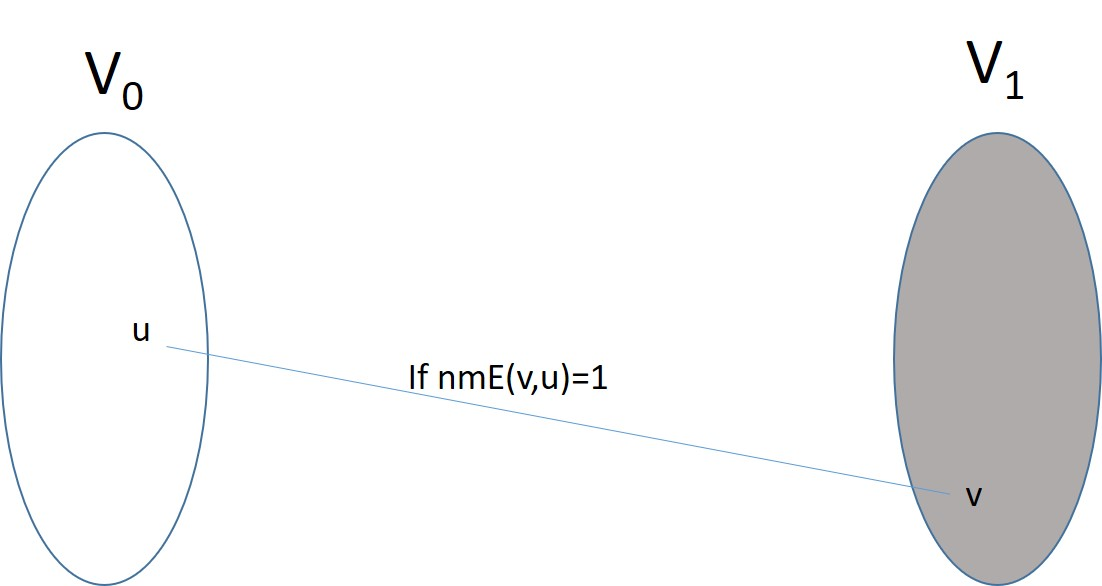
\includegraphics[width=0.8\textwidth]{fig4.jpg}}}
\caption{Illustrating the construction of Theorem~\ref{nmE2RSO:prop}.}
\label{nmE2RSO:fig}
\end{figure}



\BT[Using a quasi-orthogonal non-malleable two-source extractor to
obtain a $\Omega(2^\ell)$-robustly self-ordered $O(2^\ell)$-vertex graph]
\label{nmE2RSO:prop}
For a constant $\e\in(0,0.5)$ varying $\ell\geq k$
such that $k\leq\ell-2+\log_2(0.5-\e)=\ell-O(1)$,
%
%
suppose that ${\nmE}:[2^\ell]\times[2^\ell]\to\bitset$
is a quasi-orthogonal {\em(with error $\e$)}
non-malleable two-source $(k,\e)$-extractor.
Then, the $2^{\ell+1}$-vertex graph $G=(V_1\cup V_0,E)$
such that $V_\sigma=\{\ang{\sigma,i}\!:\!i\!\in\![2^\ell]\}$
and
\begin{equation}\label{nmE2RSO:eq}
E\;=\;\left\{\{\ang{1,i},\ang{0,j}\}\!:\!\nmE(i,j)\!=\!1\right\}
\cup \binom{V_1}{2}
\end{equation}
%
%
is $\Omega(|V_1\cup V_0|)$-robustly self-ordered.
%
Furthermore, the claim holds even if
the non-malleability condition {\rm(i.e., \eqref{nm-extractor:eq})}
holds only for permutations $f$ and $g$ that have no fixed-points.
\ET
Indeed, the first set of edges, denoted $E'$, corresponds to
a bipartite graph between $V_1$ and~$V_0$ that is determined by $\nmE$,
and the second set corresponds to a $2^\ell$-vertex clique
(see Figure~\ref{nmE2RSO:fig}).
Note that the extraction parameters are extremely weak;
that is, the min-entropy may be very high (i.e., $k=\ell-O(1)$),
the error may be an arbitrary non-trivial constant (i.e., $\e<1/2$),
and we only extract one bit (i.e., $m=1$).
\medskip

\BPF
Let $V=V_1\cup V_0$,
and consider an arbitrary (non-trivial) permutation $\mu:V\to V$.
Intuitively, if $\mu$ maps a vertex of $V_1$ to $V_0$,
then the difference in degrees of vertices in the two sets
(caused by the clique edges) contributes
at least $(2^\ell-1)-2\e\cdot2^\ell$ units
to the symmetric difference between~$G$ and~$\mu(G)$,
where here we use the first quasi-orthogonality condition.
On the other hand,
if $\mu$ maps $\ang{1,i}\in V_1$ to $V_1\setminus\{\ang{1,i}\}$,
then the difference in the neighborhoods caused by the bipartite graph
contributes at least $(0.5-\e)\cdot2^{\ell}$ units to
the symmetric difference between~$G$ and~$\mu(G)$.
To prove this, we distinguish between the case that $\mu$
has relatively few non-fixed-points (in either $V_0$ or $V_1$),
which is analyzed using the second quasi-orthogonality condition,
and the case that $\mu$ has relatively many non-fixed-points
(in both $V_0$ and $V_1$),
which is analyzed using the non-malleability condition.
Details follow.

Let $T=\{v\!\in\!V\!:\!\mu(v)\neq v\}$ denote
the set of non-fixed-points of $\mu$.
Then, we consider two types of vertices:
Those that belong to the set
$T'=\bigcup_{\sigma\in\bitset}
  \{v\!\in\!V_\sigma\!:\!\mu(v)\not\in V_{\sigma}\}\subseteq T$
and those that belong to $T\setminus T'$.
The threshold for distinguishing these cases is set
to $K=(0.5-\e)\cdot2^{\ell-2}=\Omega(|V|)$.
%
%

\BDes
%
\item[{\em Case 1}:] $|T'|\geq K$.

(This refers to the case that many vertices are mapped by $\mu$
to the opposite side of the bipartite graph $(V,E')$,
where `many' means $\Omega(|V|)$.)

Each vertex in $T'$ contributes $(1-2\e)\cdot2^\ell-1$
units to the symmetric difference between~$G$ and~$\mu(G)$,
because the degree of each vertex in $V_1$
is at least $(2^{\ell}-1)+(0.5-\e)\cdot2^\ell$,
whereas the degree of each vertex in $V_0$
is at most $(0.5+\e)\cdot2^\ell$,
where we use the first quasi-orthogonality condition,
which implies that the number of bipartite edges incident
at each vertex is at least $(0.5-\e)\cdot2^\ell$
and at most $(0.5+\e)\cdot2^\ell$.

Hence, the symmetric difference between~$G$ and $\mu(G)$ is at least
$((1-2\e)\cdot2^\ell-1)\cdot|T'|=\Omega(|V|)\cdot|T'|$,
since $2^\ell=\Omega(|V|)$.
Using the case's hypothesis,
we have $|T'|=\Omega(|V|)=\Omega(|T|)$,
which means that in this case
the difference between~$G$ and $\mu(G)$ is $\Omega(|V|)\cdot|T|$.

We stress that the difference between~$G$ and $\mu(G)$
is at least $\Omega(|V|)\cdot|T'|$
also if the case hypothesis does not hold.

%
\item[{\em Case 2}:] $|T'|<K$.

(This refers to the case that few vertices are mapped by $\mu$
to the opposite side of the bipartite graph $(V,E')$,
where `few' means less than $K\leq|V|/20$ (assuming $\e\leq0.1$).)

For every $\sigma\in\bitset$,
let $V'_\sigma=V_\sigma\cap\imu(V_\sigma)$ and $T_\sigma=V'_\sigma\cap T$.
%
Indeed, $(T',T_0,T_1)$ is a three-way partition of $T$.
%
%
Note that the size of the symmetric difference between~$G$ and $\mu(G)$
is lower-bounded by
\begin{equation}\label{diff-vs-nmE:eq}
\left|\{(v,u)\in V'_1\times V'_0:\nmE(\mu(v),\mu(u))\neq\nmE(v,u)\}\right|,
\end{equation}
since, for any $(v,u)\in V'_1\times V'_0$,
it holds that $\mu(v)$ neighbors $\mu(u)$ in~$G$
if and only if $\nmE(\mu(v),\allowbreak\mu(u))=1$,
whereas $\mu(v)$ neighbors $\mu(u)$ in $\mu(G)$
if and only if $v$ neighbors $u$ in~$G$
which holds if and only if $\nmE(v,u)=1$.
%
%
%
%
%
%
%
%
%
%
%

We consider two sub-cases according to
whether or not $\min(|T_0|,|T_1|)$ is relatively large.
The threshold for distinguishing these sub-cases
is also set to $K=(0.5-\e)\cdot2^{\ell-2}$;
note that $K=\Omega(|V|)$ and $K\geq2^k$.


\BDes
%
\item[{\em Case 2.1}:] $\min(|T_0|,|T_1|)<K$.

In this case we shall use
the (second condition of) quasi-orthogonality of $\nmE$.

Suppose, without loss of generality, that $|T_0|\leq|T_1|$,
which implies $|T_0|<K$.
%
Then, the contribution of
each vertex $v\in T_1$ to \eqref{diff-vs-nmE:eq} equals
\begin{eqnarray*}
\lefteqn{|\{u\in V'_0:\nmE(\mu(v),\mu(u))\neq\nmE(v,u)\}|} \\
&\geq& |\{u\in V'_0:\nmE(\mu(v),u)\neq\nmE(v,u)\}| - |T_0| \\
&\geq& |\{u\in V_0:\nmE(\mu(v),u)\neq\nmE(v,u)\}|-|T'|-|T_0| \\
%
&\geq& (0.5-\e)\cdot2^\ell-2\cdot K \\
&=& (0.5-\e)\cdot2^{\ell-1}
\end{eqnarray*}
where the first inequality uses $\mu(u)=u$ for $u\in V'_0\setminus T_0$,
the second inequality uses $|V'_0|\geq|V_0|-|T'|$,
the third inequality uses $\mu(v)\neq v$
along with the (second condition of) quasi-orthogonality of $\nmE$
(and the hypotheses regarding $|T'|$ and $|T_0|$),
and the equality is due to $K=(0.5-\e)\cdot2^{\ell-2}$.


Hence, in this case,
the total contribution to \eqref{diff-vs-nmE:eq} is
$(0.5-\e)\cdot2^{\ell-1}\cdot|T_1|$,
which is $\Omega(|V|)\cdot(|T|-|T'|)$,
since $|T_1|\geq(|T|-|T'|)/2$.
%

%
\item[{\em Case 2.2}:] $\min(|T_0|,|T_1|)\geq K$.

In this case we shall use the non-malleable feature of $\nmE$.

Specifically, for each $\sigma\in\bitset$,
let $\mu_\sigma$ denote the restriction of $\mu$ to $T_\sigma$.
%
%
Essentially, using $K\geq2^k$,
the non-malleability condition of the $(k,\e)$-extractor $\nmE$ implies
%
$$\left|\left\{(i,j)\in T_0\times T_1:
            \nmE(i,j)\neq\nmE(\mu_0(i),\mu_1(j))\right\}\right|
  \geq(0.5-\e)\cdot|T_0|\cdot|T_1|.$$
This can be seen by
letting $X$ and $Y$ be uniform over $T_0$ and $T_1$, respectively.
(Also, for sake of formality, we extend $\mu_0$ and $\mu_1$
(which have no fixed-points)
to (arbitrary) derangements $f$ and $g$, respectively.)
\footnote{Note that we may assume, w.l.o.g.,
that $|T_\sigma\cup\mu(T_\sigma)|\leq|V_\sigma|-2$.}
%
In this case, the non-malleability condition implies that
the distribution $(\nmE(X,Y),\nmE(f(X),g(Y)))$
is $\e$-close to $(U_1,\nmE(f(X),g(Y)))$,
which implies that $\prob[\nmE(X,Y)\neq\nmE(\mu_0(X),\mu_1(Y))]$
is at least $\prob[U_1\neq\nmE(\mu_0(X),\mu_1(Y))]-\e=0.5-\e$.
%
%
%
%
%
%
%
%
%
%
%
%
%
%
%
%
%
%
%
%
%
%

%
%
Hence, in this case,
the total contribution to \eqref{diff-vs-nmE:eq} is
$(0.5-\e)\cdot|T_0|\cdot|T_1|=\Omega(|V|)\cdot(|T|-|T'|)$,
where we use $\min(|T_0|,|T_1|)=\Omega(|V|)$
and $|T_0|+|T_1|=|T|-|T'|$.
\EDes
Hence, in both sub-cases, the difference between~$G$ and $\mu(G)$
is $\Omega(|V|)\cdot(|T|-|T'|)$.
\EDes
Recall that (by the last comment at Case~1)
the difference between~$G$ and $\mu(G)$
is $\Omega(|V|)\cdot|T'|$.
Combining this lower-bound with the conclusion of Case~2,
the difference between~$G$ and $\mu(G)$ is $\Omega(|V|)\cdot|T|$.
\EPF


\paragraph{Digest:}
Note that the quasi-orthogonality of $\nmE$ was used in Cases~1 and~2.1,
whereas the non-malleability of $\nmE$ (w.r.t derangements)
was used in Case~2.2. In particular, Case~1 only uses the
first condition of quasi-orthogonality, and does so in order to infer
that the degrees of all vertices in the bipartite graph
are approximately equal.
In Case~2.1 the second quasi-orthogonality condition
is used in order to assert that the neighborhoods of two
different vertices in $V_\sigma$ are significantly different.
This is useful only when the number of non-fixed-points in $V_{1-\sigma}$
is relatively small.
When the number of non-fixed-points in both $V_\sigma$'s is large
but few vertices are mapped to the other side (i.e., $|T'|\ll|T|$),
%
we only use Case~2.2, which does not refer to quasi-orthogonality at all.
Hence, we have the following~--


\BR[A special case of Theorem~\ref{nmE2RSO:prop}]
\label{nmE2RSO:rem}
For bipartite graphs $G=(V,E)$ such that $V=V_0\cup V_1$
and $E\subseteq V_0\times V_1$,
we consider the special case of robust self-ordering
that refers only to permutations $\mu:V\to V$
that are derangements that preserve the bipartition of $V$
{\rm(i.e., $\mu$ has no fixed-points and $\mu(V_0)=V_0$)}.
\footnote{That is, the requirement regarding the symmetric difference
between~$G$ and $\mu(G)$ is made only for permutations $\mu$
that have no fixed-points and satisfy $\mu(V_0)=V_0$.}
%
%
In this case, assuming {\rm(only)} that $\nmE$ is
a non-malleable two-source $(\ell,\e)$-extractor
{\rm(i.e., the case of $k=\ell$)},
implies that, for any such $\mu$,
the size of the symmetric difference between~$G$ and $\mu(G)$
is $(0.5\pm\e)\cdot|V_0|\cdot|V_1|$.
Furthermore, the claim holds even if the non-malleability condition
holds only for permutations $f$ and $g$ that have no fixed-points
{\em(i.e., derangements)},
and the quasi-orthogonality condition is not necessary.
Note that the proof of Theorem~\ref{nmE2RSO:prop} simplifies,
since $T'=\emptyset$ and $T_\sigma=V_\sigma=V'_\sigma$ hold,
and the size of the symmetric difference between~$G$ and $\mu(G)$
equal the quantity in \eqref{diff-vs-nmE:eq}.
\ER
Interestingly, the special case of Theorem~\ref{nmE2RSO:prop}
asserted in Remark~\ref{nmE2RSO:rem} can be reversed in the
sense that a bipartite graph that is robustly self-ordered
in the foregoing restricted sense is actually
a non-malleable two-source $(\ell,0.5-\Omega(1))$-extractor
(w.r.t derangement).
In the following result $\e$ is an arbitrary constant (in $(0,0.5)$),
whereas~$G$ varies and $o(1)$ vanishes with~$|V|$.

\BP[A reversal of the special case of Theorem~\ref{nmE2RSO:prop}
(i.e., of Remark~\ref{nmE2RSO:rem})]
\label{reverse-nmE2RSO:prop}
Let $G=(V_0\cup V_1,E)$ be a bipartite graph
such that $|V_0|=|V_1|$ and $E\subseteq V_0\times V_1$.
%
%
Let $V=V_0\cup V_1$, and
suppose that for every derangement $\mu:V\to V$
such that $\mu(V_0)=V_0$ it holds that the
size of the symmetric difference between~$G$ and $\mu(G)$
is $(0.5\pm\e)\cdot|V_0|\cdot|V_1|$.
Then, $F:V_0\times V_1\to\bitset$
such that $F(x,y)=1$ if and only if $\{x,y\}\in E$
is a non-malleable two-source $(\ell,\e+{\sqrt{2\e}}+o(1))$-extractor
w.r.t derangement.
\footnote{That is, the non-malleability condition
(i.e., \eqref{nm-extractor:eq}) is guaranteed
only for permutations $f$ and $g$ that have no fixed-points.}
\EP
Needless to say, the claim holds also if~$G$ is augmented
by complete graph on the vertex-set~$V_1$.
Note that we lose a $\sqrt{2\e}+o(1)$ term in the reversal.
%
%
\medskip

%
%
%
%
%
%
%
%
%
%
%
%
%
%
%
%
%
%
%

\BPF
Let $(f,g)$ and $(X,Y)$ be as in Definition~\ref{nmExtractor:def},
and note that in this case $X$ and $Y$ are independent distributions
that are each uniformly distributed on $[2^\ell]$.
%
%
%
Define $\mu:V\to V$ such that $\mu(z)=f(z)$ if $z\in V_0$
and $\mu(z)=g(z)$ otherwise, and note that $\mu$ is a derangement
that preserves the partition of $V$.
Recall that $(\mu(x),\mu(y))$ contributes to the symmetric difference
between~$G$ and $\mu(G)$ if and only if $F(\mu(x),\mu(y))\neq F(x,y)$,
since $\mu(x)$ is connected to $\mu(y)$ in~$\mu(G)$
if and only if $x$ is connected to $y$ in~$G$.
Hence, by the hypothesis, we have
\begin{equation}\label{reverse-nmE2RSO:eq}
\prob[F(X,Y)\neq F(\mu(X),\mu(Y))]=0.5\pm\e.
\end{equation}
Letting
$p_{\sigma,\tau}^\mu\eqdef\prob[(F(X,Y),F(\mu(X),\mu(Y)))\!=\!(\sigma,\tau)]$,
we have $p_{0,1}^\mu+p_{1,0}^\mu=0.5\pm\e$,
and using the fact that $(X,Y)$ and $(\mu(X),\mu(Y))$
are identically distributed we have $p_{1,0}^\mu=p_{0,1}^\mu$
(since $p_{1,1}^\mu+p_{1,0}^\mu=p_{1,1}^\mu+p_{0,1}^\mu$).
Hence, $p_{0,1}^\mu=0.25\pm0.5\e$.
Lastly, we show that $p_{1,1}^\mu+p_{1,0}^\mu=0.5\pm{\sqrt{\e/2}}+o(1)$,
and conclude that $p_{1,1}^\mu=0.25\pm(0.5\e+{\sqrt{\e/2}}+o(1))$;
it follows that $F$ is
a non-malleable (two-source) $(\ell,\e+{\sqrt{2\e}}+o(1))$-extractor.
%

To show that $p_{1,1}^\mu+p_{1,0}^\mu=0.5\pm{\sqrt{\e/2}}+o(1)$,
we first note that $p\eqdef p_{1,1}^\mu+p_{1,0}^\mu=\prob[F(X,Y)\!=\!1]$
is actually oblivious of $\mu$.
%
Hence, by considering a random derangement $\mu$ that preserves $V_0$
(i.e., $\mu(V_0)=V_0$), we observe that,
with overwhelmingly high probability (over the choice of $\mu$),
it holds that $\{(x,y)\!\in\!V_0\times V_1\!:\!F(x,y)\neq F(\mu(x),\mu(y))\}$
has size $(2p(1-p)\pm o(1))\cdot|V_0|\cdot|V_1|$.
%
%
%
%
%
Confronting this with \eqref{reverse-nmE2RSO:eq},
we infer that $p=0.5\pm({\sqrt{\e/2}}+o(1))$.
%
%
\EPF


\paragraph{Corollary.}
Combining Theorem~\ref{nmE2RSO:prop}
with the non-malleable two-source extractors of~\cite[Thm.~1]{CGL},
while using Proposition~\ref{nmE-made-nice:prop},
we obtain an efficient construction
of $\Omega(n)$-robustly self-ordered graphs
(alas not a strongly explicit (aka locally computable) one).

\BT[Constructing $\Omega(n)$-robustly self-ordered $n$-vertex graphs]
\label{dense-rso1:thm}
There exist an algorithm that, on input $n$,
works in $\poly(n)$-time and outputs an explicit description of
an $\Omega(n)$-robustly self-ordered $O(n)$-vertex graph.
Furthermore, each vertex in this graph has degree
at least $0.24\cdot n$ and at most $0.76\cdot n$.
\ET
The degree bounds follow by observing that the vertices
in the graph described in Theorem~\ref{nmE2RSO:prop}
have degree at least $(0.5-\e)\cdot n/2$
and at most $(1.5+\e)\cdot n/2$,
whereas~\cite[Thm.~1]{CGL} provides for $\e=o(1)$.



















































































































%
%
%
%

\subsection{The second construction}
\label{dense:rso2:sec}
Combining Theorem~\ref{nmE2RSO:prop}
with the non-malleable two-source extractors of~\cite[Thm.~1]{CGL},
while using Proposition~\ref{nmE-made-nice:prop},
we obtained an efficient construction
of $\Omega(n)$-robustly self-ordered $n$-vertex graphs
(see Theorem~\ref{dense-rso1:thm}).
%
%
%
Unfortunately, this construction is not locally computable
(as postulated in Theorem~\ref{dense:ithm}),
because the non-malleable two-source extractors of~\cite[Thm.~1]{CGL}
are not quasi-orthogonal and the transformation
of Proposition~\ref{nmE-made-nice:prop} runs in time
that is polynomial in the size of the resulting graph.

To avoid the foregoing transformation and prove Theorem~\ref{dense:ithm},
we employ a variant on the construction presented
in Theorem~\ref{nmE2RSO:prop}.
Rather than connecting two sets of vertices using
a bipartite graph that corresponds to
a {\em quasi-orthogonal}\/ non-malleable two-source extractor,
we connect three sets of vertices such that one pair
of vertex-sets is connected by a (not necessarily quasi-orthogonal)
non-malleable two-source extractor, whereas the other two pairs
are connected by bipartite graphs that are merely quasi-orthogonal.
In analogy to the definition of a quasi-orthogonal (two-source) extractor,
we say that a bipartite graph on the vertex-set $X\cup Y$
is {\sf quasi-orthogonal} (with error $\e$)
if the following two conditions hold regarding
its adjacency predicate $B:X\times Y\to\bitset$:
\BE
\item
{\em The degree of each vertex is approximately half
the number of the vertices on the other side}:
For each $x\in X$ (resp., $y\in Y$), it holds that
$|\{y\!\in\!Y\!:\!B(x,y)\!=\!1\}|=(0.5\pm\e)\cdot|Y|$
(resp., $|\{x\!\in\!X\!:\!B(x,y)\!=\!1\}|=(0.5\pm\e)\cdot|X|$).
%
%
\item
%
%
{\em For each pair of vertices on one side,
approximately half the vertices on the other side
neighbor exactly one of the vertices in the pair}:
For every $x\neq x'\in X$, it holds that
$|\{y\!\in\!Y\!:\!B(x,y)\!\neq\!B(x',y)\}|=(0.5\pm\e)\cdot|Y|$.
%
%
Similarly, for $y\neq y'\in Y$.
\EE
We note that inner-product (mod~2) extractor,
denoted $E_2:\bitset^\ell\times\bitset^\ell\to\bitset$,
corresponds to a quasi-orthogonal bipartite graph for
the case $X=Y=\bitset^\ell\setminus\{0^\ell\}$.
We will however need quasi-orthogonal bipartite graphs with
different-sized sides, which can be obtained by a simple variant.
Specifically, for the case of $X=\bitset^\ell\setminus\{0^\ell\}$
and $Y=\bitset^{\ell+2}\setminus\{0^{\ell+2}\}$,
we use the function $B(x,y)=E_2(G(x),y)$,
where $G:\bitset^\ell\to\bitset^{\ell+2}$
is a small-bias generator that satisfies $G(x)\neq0^{\ell+2}$
and $G(x)\neq G(x')$ for every $x\neq0^\ell$ and $x'\neq x$
(see Proposition~\ref{nice-bipartite:prop},
and note that $G(a,b,c,d)=(a,b,c,d,E_2(a,b),E_2(c,d))$ will do).
We stress that the foregoing construction is strongly explicit
(i.e., locally computable).
%
%
%


We shall also assume that the (bipartite graph corresponding to the)
non-malleable extractor ${\nmE}:[2^\ell-1]\times[2^\ell-1]\to\bitset$
has {\em linear degrees}\/ in the sense that for every $x$ it holds that
$|\{y\!\in\![2^\ell-1]\!:\!\nmE(x,y)\!=\!1\}|\geq\e'\cdot2^\ell$
for some constant $\e'>0$.
This can be enforced by starting with an arbitrary
non-malleable two-source $(k,\e')$-extractor
(e.g., the one of~\cite[Thm.~1]{CGL})
and resetting pairs in $m=\e'\cdot2^\ell$ fixed perfect matchings to~1
(i.e., for each $(x,y)$ in one of these matching, we reset $\nmE(x,y)\gets1$).
\footnote{For example, we may use the matchings $\{(z,z+i):z\in[2^\ell-1]\}$
for $i\in[m]$, where addition is mod~$2^\ell-1$.
Furthermore, starting from an extractor that is defined
over $\ell$-bit strings, we may omit one of these strings
(and obtain an extractor defined over $[2^\ell-1]$).}
%
%
%
%
This increases the error of the extractor by an additive
term of $m/2^k=2^{\ell-k}\cdot\e'$, which we can afford
(e.g., $\e'=0.01$ and $k=\ell-4$,
yields extraction error $\e<0.2$).
We stress that this transformation preserves
polynomial-time computability of the extracting function.
%
%
%
%
%
%
%
%
%
%
%
%
%
%
%
%
%
%
%
%
%
%
%

\BT[Using a non-malleable two-source extractor with linear degrees to
obtain a $\Omega(2^\ell)$-robustly self-ordered $O(2^\ell)$-vertex graph]
%
%
%
%
%
%
%
\label{nmE2RSO-tri:thm}
%
%
%
%
%
%
For any constants $\e,\e'\in(0,0.5)$ and varying $k\leq\ell-4$,
where $\ell\in\N$,
suppose that ${\nmE}:[2^\ell-1]\times[2^\ell-1]\to\bitset$
is a non-malleable two-source $(k,\e)$-extractor
such that for every $x$ it holds that
$|\{y\!\in\![2^\ell-1]\!:\!\nmE(x,y)\!=\!1\}|>\e'\cdot2^\ell$.
%
Further suppose that $B:[2^\ell-1]\times[2^{\ell+2}-1]\to\bitset$
is quasi-orthogonal with error $0.1\cdot\e'$.
Then, the $(6\cdot2^{\ell}-3)$-vertex graph $G=(V_0\cup V_1\cup V_2,E)$
such that $V_\sigma=\{\ang{\sigma,i}\!:\!i\!\in\![2^{\ell_\sigma}-1]\}$,
where $\ell_0=\ell_1=\ell$ and $\ell_2=\ell+2$,
and
\begin{equation}\label{nmE2RSO-tri:eq}
E\;=\;\left\{\{\ang{1,i},\ang{0,j}\}\!:\!\nmE(i,j)\!=\!1\right\}
\cup\left\{\{
    \ang{\sigma,i},\ang{2,j}\}\!:\!B(i,j)\!=\!1,\sigma\in\bitset
       \right\}
\cup \binom{V_1}{2}
\cup \binom{V_2}{2}
\end{equation}
%
%
is $\Omega(|V|)$-robustly self-ordered, where $V=V_0\cup V_1\cup V_2$.
%
%
%
%
%
%
%
%
%
%
%
Furthermore, each vertex in this graph has degree
at least $0.3\cdot|V|$ and at most $0.9\cdot|V|$.
Moreover, the claim holds even if
the non-malleability condition {\rm(i.e., \eqref{nm-extractor:eq})}
holds only for permutations $f$ and $g$ that have no fixed-points.
\ET
Using the foregoing ingredients
(including the non-malleable extractor of~\cite[Thm.~1]{CGL}),
Theorem~\ref{dense:ithm} follows
(see also Remark~\ref{dense:rso:all-n's:rem}).
%
Looking at \eqref{nmE2RSO-tri:eq}, note that
the first set of edges corresponds to a bipartite
graph between $V_1$ and $V_0$ that is determined by $\nmE$,
the second set corresponds the bipartite graphs
between $V_\sigma$ (for $\sigma\in\bitset$) and $V_2$
that are determined by $B$,
and the other two sets correspond to cliques on $V_1$ and on $V_2$
(see Figure~\ref{nmE2RSO-tri:fig}).
\medskip


\begin{figure}
\centerline{\mbox{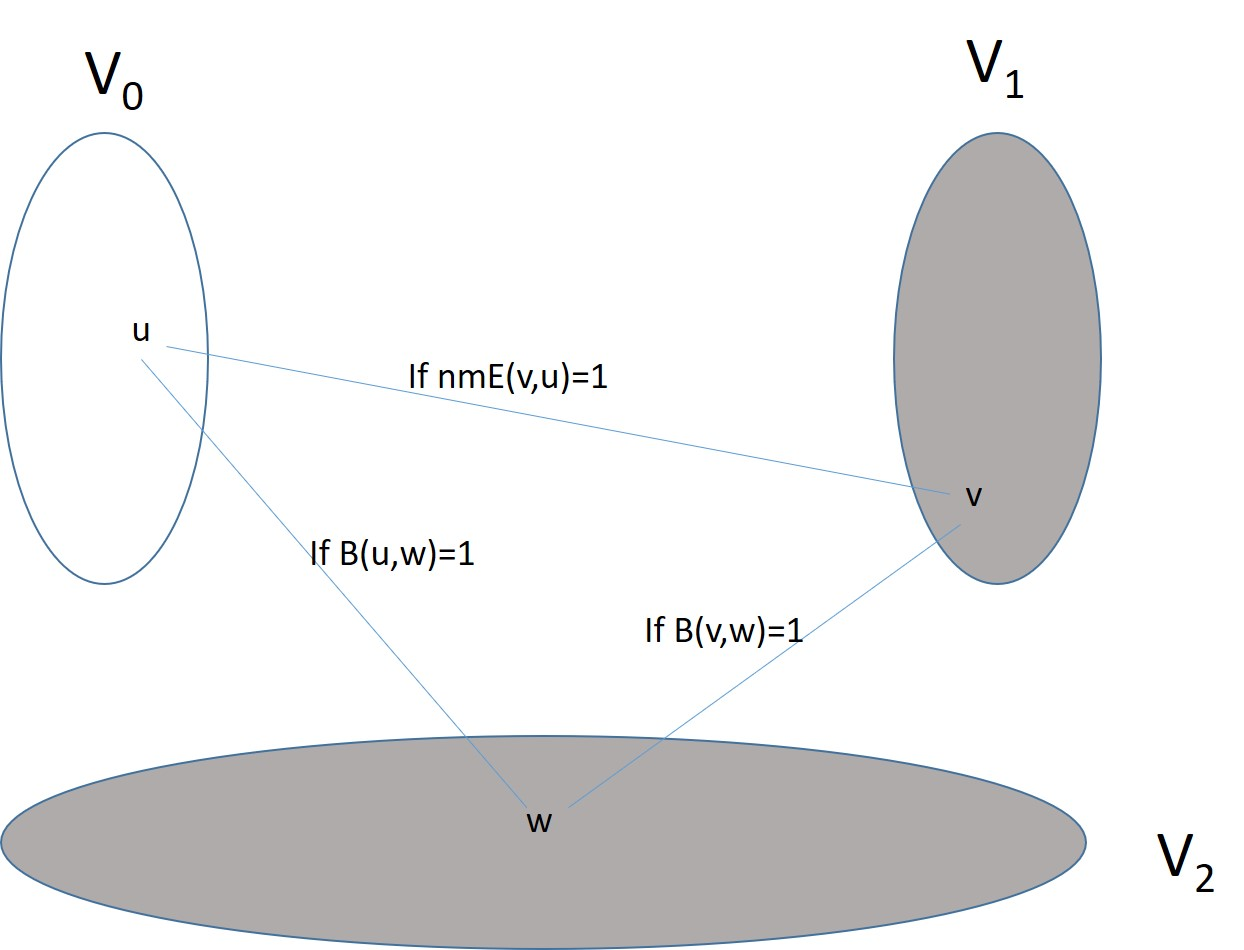
\includegraphics[width=0.8\textwidth]{fig5.jpg}}}
\caption{Illustrating the construction of Theorem~\ref{nmE2RSO-tri:thm}.}
\label{nmE2RSO-tri:fig}
\end{figure}


\BPF
Recall that $V=V_0\cup V_1\cup V_2$, and
consider an arbitrary (non-trivial) permutation $\mu:V\to V$.
Intuitively, if $\mu$ maps a vertex of $V_0$ (or $V_1$) to $V_2$,
then the difference in the degrees of the vertices in the two sets
(caused by the $|V_2|$-clique edges) contributes $\Omega(|V|)$
units to the symmetric difference between~$G$ and $\mu(G)$,
where here we use the first quasi-orthogonality condition of $B$.
A similar argument, which uses the $V_1$-clique edges
and relies on the linear degrees of $\nmE$,
applies to a vertex of $V_\sigma$ mapped to $V_{1-\sigma}$
for any $\sigma\in\bitset$.
On the other hand, if for some $\sigma\in\{0,1,2\}$
the bijection $\mu$ maps $\ang{\sigma,i}\in V_\sigma$
to $V_\sigma\setminus\{\ang{\sigma,i}\}$,
then the difference in the neighborhoods caused by one
of the two relevant bipartite graphs contributes $\Omega(|V|)$
units to the symmetric difference between~$G$ and $\mu(G)$.
Here, we distinguishes between
the case that~$\mu$ has relatively few non-fixed-points
in either $V_0$ or $V_1$,
which is analyzed using the second quasi-orthogonality condition of $B$,
and the case that $\mu$ has relatively many non-fixed-points
in both $V_0$ and $V_1$,
which is analyzed using the non-malleability condition of $\nmE$.
Indeed, the structure of the proof is similar to the one
of Theorem~\ref{nmE2RSO:prop}, but the details are different
in many aspects, and so we provide them below.
%

Let $T=\{v\!\in\!V\!:\!\mu(v)\neq v\}$ denote
the set of non-fixed-points of $\mu$.
Then, we consider two types of vertices:
Those that belong to the set
$T'=\bigcup_{\sigma\in\{0,1,2\}}
  \{v\!\in\!V_\sigma\!:\!\mu(v)\not\in V_{\sigma}\}\subseteq T$
%
and those that belong to $T\setminus T'$.
The threshold for distinguishing these cases is set
to $K=(0.5-0.1\cdot\e')\cdot|V_0|/4=\Omega(|V|)$.
\footnote{The threshold is set depending on the quasi-orthogonality
error of $B$. In the proof of Theorem~\ref{nmE2RSO:prop},
the threshold was set depending on the quasi-orthogonality
error of $\nmE$ (which equaled its extraction error).}
%
%
%
Recall that $\e$ denotes the extraction error of $\nmE$,
whereas $\e'$ is the fractional degree bound associated
with its linear degrees feature,
and $0.1\cdot\e'$ is the quasi-orthogonality error of~$B$.


\BDes
%
\item[{\em Case 1}:] $|T'|\geq K$.

(This refers to the case that many vertices are mapped by $\mu$
to a different part of the three-way partition $(V_0,V_1,V_2)$ of $V$,
where `many' means $\Omega(|V|)$.)

Each vertex in $T'$ contributes $\Omega(|V|)$ units
to the symmetric difference between~$G$ and $\mu(G)$,
because of the differences in the degrees of vertices
in the three parts. Specifically:
\BI
\item Vertices in $V_2$ have degree at least
$(|V_2|-1)+(0.5-0.1\e')\cdot(|V_0|+|V_1|)>(5-0.2\e')\cdot|V_0|-O(1)$,
%
where the first term is due to the clique edges
and the second term is due to the bipartite graphs
connecting $V_2$ to $V_0$ and to $V_1$
(and relies on the first quasi-orthogonality condition of $B$).
\item Vertices in $V_0$ have degree at most
$|V_1|+(0.5+0.1\e')\cdot|V_2|<(3+0.4\e')\cdot|V_0|+O(1)$,
%
where the first term is due to the edges (determined by $\nmE$)
connecting $V_0$ to $V_1$ and the second term is due to
the bipartite graph connecting $V_0$ to $V_2$.
\item
Vertices in $V_1$ have degree at least
$(|V_1|-1)+\e'\cdot|V_0|+(0.5-0.1\e')\cdot|V_2|>(3+0.6\e')\cdot|V_0|-O(1)$
%
and at most
$(|V_1|-1)+|V_0|+(0.5+0.1\e')\cdot|V_2| < (4+0.4\e')\cdot|V_0|$.
%
In both cases, the first term is due to clique edges,
the second term is due to the edges connecting $V_1$ to $V_0$
(as determined by $\nmE$), and the third term is due to
the edges connecting $V_1$ to $V_2$ (as determined by $B$).
The crucial fact is that the linear degrees of $\nmE$ provides
a non-trivial lower bound (of $\e'\cdot|V_0|$) on the second term.
\EI
Hence, the difference in the degrees of vertices in the different
parts is at least $0.2\e'\cdot|V_0|-O(1)$, where the minimum
is due to the difference between the degrees of vertices in $V_1$
and the degrees of vertices in $V_0$.

It follows that the symmetric difference between~$G$ and $\mu(G)$
is at least $(0.2\e'\cdot|V_0|-O(1))\cdot|T'|=\Omega(|V|)\cdot|T'|$,
since $|V_0|=\Omega(|V|)$ and $\e'=\Omega(1)$.
Using the case's hypothesis,
we have $|T'|=\Omega(|V|)=\Omega(|T|)$,
which means that in this case
the difference between~$G$ and $\mu(G)$ is $\Omega(|V|)\cdot|T|$.

We stress that the difference between~$G$ and $\mu(G)$
is at least $\Omega(|V|)\cdot|T'|$
also if the case hypothesis does not hold.

%
\item[{\em Case 2}:] $|T'|<K$.

(This refers to the case that few vertices are mapped by $\mu$
to a different part of the three-way partition $(V_0,V_1,V_2)$ of $V$.)

For every $\sigma\in\{0,1,2\}$,
let $V'_\sigma=V_\sigma\cap\imu(V_\sigma)$ and $T_\sigma=V'_\sigma\cap T$.
Indeed, $(T',T_0,T_1,T_2)$ is a four-way partition of $T$.
Note that the size of the symmetric difference between~$G$ and $\mu(G)$
is lower-bounded by
\begin{equation}\label{diff-vs-nmE-tri:eq}
\begin{array}{ll}
&\left|\{(v,u)\in V'_1\times V'_0:\nmE(\mu(v),\mu(u))\neq\nmE(v,u)\}\right| \\
&+\;\left|\{(v,u)\in V'_1\times V'_2:B(\mu(v),\mu(u))\neq B(v,u)\}\right| \\
&+\;\left|\{(v,u)\in V'_0\times V'_2:B(\mu(v),\mu(u))\neq B(v,u)\}\right|,
\end{array}
\end{equation}
since, for any $(v,u)\in V'_1\times V'_0$,
it holds that $\mu(v)$ neighbors $\mu(u)$ in~$G$
if and only if $\nmE(\mu(v),\allowbreak \mu(u))=1$,
whereas $\mu(v)$ neighbors $\mu(u)$ in $\mu(G)$
if and only if $v$ neighbors $u$ in~$G$
which holds if and only if $\nmE(v,u)=1$.
Ditto for the other two cases.
%
%
%
%
%
%
%
%
%
%
%

We consider two sub-cases according to
whether or not $\min(|T_0|,|T_1|)$ is relatively large.
The threshold for distinguishing these sub-cases is also set
to $K=(0.5-0.1\cdot\e')\cdot|V_0|/4$;
note that $K=\Omega(|V|)$ and $K>0.1\cdot|V_0|>2^{\ell-4}\geq2^k$.
%
%
%
%

\BDes
\item[{\em Case 2.1}:] $\min(|T_0|,|T_1|)<K$.
%
%

In this case we shall use the quasi-orthogonality of $B$.

Suppose, without loss of generality, that $|T_0|\leq|T_1|$,
which implies $|T_0|<K$. 

Depending on the relative sizes of $T_1$ and $T_2$,
we shall use either the quasi-orthogonal bipartite graph
between $V_1$ and $V_2$
or the quasi-orthogonal bipartite graph between $V_2$ and $V_0$.
\BE
\item
If $|T_1|>|T_2|$, then we consider
the quasi-orthogonal bipartite graph between $V_1$ and $V_2$.
%
The contribution of
each vertex $v\in T_1$ to \eqref{diff-vs-nmE-tri:eq} equals
\begin{eqnarray*}
\lefteqn{|\{u\in V'_2:B(\mu(v),\mu(u))\neq B(v,u)\}|} \\
&\geq& |\{u\in V'_2:B(\mu(v),u)\neq B(v,u)\}| - |T_2| \\
&>& |\{u\in V_2:B(\mu(v),u)\neq B(v,u)\}|-|T'|-|T_1| \\
&\geq& (0.5-0.1\cdot\e')\cdot|V_2|-K-|V_0| \\
&\geq& (4-0.25)\cdot(0.5-0.1\e')\cdot|V_0|-|V_0| \\
%
%
%
%
%
%
%
&>& 0.6\cdot|V_0|
%
%
%
%
%
%
%
\end{eqnarray*}
where the first inequality uses $\mu(u)=u$ for $u\in V'_2\setminus T_2$,
the second inequality uses $|V'_2|\geq|V_2|-|T'|$
and the hypothesis $|T_2|<|T_1|$,
the third inequality uses $\mu(v)\neq v$
along with the (second condition of) quasi-orthogonality of $B$
%
(and the hypotheses $|T'|<K$
and the fact that $|T_1|\leq|V_1|=|V_0|$),
the fourth inequality uses $|V_2|>4\cdot|V_0|$ and the definition of $K$,
and the last inequality uses $\e'<0.5$.
%

So the total contribution in this sub-case is
$|T_1|\cdot\Omega(|V|)\geq(|T|-|T'|)\cdot\Omega(|V|)$,
since $|T_1|\geq\max(|T_0|,|T_2|)$ and $|T_0|+|T_1|+|T_2|=|T|-|T'|$.
\item
If $|T_1|\leq|T_2|$, then
we consider the quasi-orthogonal bipartite graph between $V_2$ and $V_0$.
%
The contribution of
each vertex $v\in T_2$ to \eqref{diff-vs-nmE-tri:eq} equals
\begin{eqnarray*}
\lefteqn{|\{u\in V'_0:B(\mu(u),\mu(v))\neq B(u,v)\}|} \\
&\geq& |\{u\in V'_0:B(u,\mu(v))\neq B(u,v)\}| - |T_0| \\
&\geq& |\{u\in V_0:B(u,\mu(v))\neq B(u,v)\}|-|T'|-|T_0| \\
&\geq& (0.5-0.1\cdot\e')\cdot|V_0|-2\cdot K \\
&=& (0.5-0.1\cdot\e')\cdot|V_0|/2
%
%
%
\end{eqnarray*}
where the first inequality uses $\mu(u)=u$ for $u\in V'_0\setminus T_0$,
the second inequality uses $|V'_0|\geq|V_0|-|T'|$,
the third inequality uses $\mu(v)\neq v$
along with the (second condition of) quasi-orthogonality of $B$
(and the hypotheses regarding $|T'|$ and $|T_0|$),
and the equality is due to $K=(0.5-0.1\cdot\e')\cdot|V_0|/4$.
%

So the total contribution in this sub-case is
$|T_2|\cdot\Omega(|V|)\geq(|T|-|T'|)\cdot\Omega(|V|)$,
since $|T_2|\geq|T_1|\geq|T_0|$.
\EE
Hence, the total contribution (of Case~2.1)
to \eqref{diff-vs-nmE-tri:eq} is $\Omega(|V|)\cdot(|T|-|T'|)$.

%
%
\item[{\em Case 2.2}:] $\min(|T_0|,|T_1|)\geq K$.

In this case we shall use the non-malleable feature of $\nmE$.

Specifically, for each $\sigma\in\bitset$,
let $\mu_\sigma$ denote the restriction of $\mu$ to $T_\sigma$.
%
%
Essentially, using $K\geq2^k$,
the non-malleability condition of the $(k,\e)$-extractor $\nmE$ implies
%
$$\left|\left\{(i,j)\in T_0\times T_1:
            \nmE(i,j)\neq\nmE(\mu_0(i),\mu_1(j))\right\}\right|
  \geq(0.5-\e)\cdot|T_0|\cdot|T_1|.$$
As in (Case 2.2 of) the proof of Theorem~\ref{nmE2RSO:prop},
this can be seen by
letting $X$ and $Y$ be uniform over $T_0$ and $T_1$, respectively.
\footnote{Recall that, formally, we also
extend $\mu_0$ and $\mu_1$ (which have no fixed-points)
to (arbitrary) derangements $f$ and $g$, respectively.
Then, the non-malleability condition implies
that $(\nmE(X,Y),\nmE(f(X),g(Y)))$ is $\e$-close to $(U_1,\nmE(f(X),g(Y)))$,
which implies that $\prob[\nmE(X,Y)\neq\nmE(\mu_0(X),\mu_1(Y))]$
is at least $\prob[U_1\neq\nmE(\mu_0(X),\mu_1(Y))]-\e=0.5-\e$.}
%
%
%
%
%
%
%
%
%
%
%
%
%
%
%
%
%
%
%
%
%
%
%

%
%
Hence, in this case,
the total contribution to \eqref{diff-vs-nmE-tri:eq} is
$(0.5-\e)\cdot|T_0|\cdot|T_1|=\Omega(|V|^2)$,
where we use $\min(|T_0|,|T_1|)=\Omega(|V|)$.
%
\EDes
Hence, in both sub-cases, the difference between~$G$ and $\mu(G)$
is $\Omega(|V|)\cdot(|T|-|T'|)$.
\EDes
Recall that (by the last comment at Case~1)
the difference between~$G$ and $\mu(G)$
is $\Omega(|V|)\cdot|T'|$.
Combining this lower-bound with the conclusion of Case~2,
the difference between~$G$ and $\mu(G)$ is $\Omega(|V|)\cdot|T|$.
%
As for the degree bounds,
note that each vertex has degree at most
$(|V_2|-1)+(0.5+0.1\e')\cdot(|V_0|+|V_1|)=\frac{5+0.2\e'}{6}\cdot|V|+O(1)$,
and at least $(0.5-0.1\e')\cdot|V_2|=\frac{2-0.4\e'}{6}\cdot|V|-O(1)$,
%
%
where maximum (resp., minimum) is obtained
by vertices in $V_2$ (resp., $V_0$).
%
\EPF

\paragraph{Digest:}
Compared to the construction used in Theorem~\ref{nmE2RSO:prop},
the construction in Theorem~\ref{nmE2RSO-tri:thm} decouples
the non-malleable feature from the quasi-orthogonality feature,
using non-malleable extractors for connecting one pair of vertex-sets
and quasi-orthogonal functions to connect the other two pairs.
The current analysis is slightly more complex because it has
to handle the fact that these features hold for different pairs.
Specifically, the quasi-orthogonality of $B$ is used in Cases~1 and~2.1,
whereas the non-malleability of $\nmE$ is used in Case~2.2.
In particular, Case~1 only uses the first condition of quasi-orthogonality,
and does so in order to infer that the degrees of all vertices
in the bipartite graph determined by $B$ are approximately equal.
In Case~2.1 the second quasi-orthogonality condition is used
in order to assert that the neighborhoods of two different vertices
in $V_\sigma$ (for every $\sigma\in\{0,1,2\}$) are significantly different.
This is useful only when the number of non-fixed-points
in the other side of the graph $B$ is relatively small.
%
%
%
%

In light of the key role that quasi-orthogonal unbalanced bipartite
graphs play in Theorem~\ref{nmE2RSO-tri:thm} and given their natural appeal,
it feel adequate to provide a general construction of these graphs,
which generalizes the construction outlined before
Theorem~\ref{nmE2RSO-tri:thm} (for the case of $\ell'=\ell+2$).
%
%
%
%


\BP[Quasi-orthogonal unbalanced bipartite graphs]
\label{nice-bipartite:prop}
For $\ell\leq\ell'$ and $S_\ell\eqdef\bitset^\ell\setminus\{0^\ell\}$
let $G:S_\ell\to S_{\ell'}$ be a small-bias generator with bias $\e$
such that $G(s)\neq G(s')$ for every $s\neq s'$,
and let $E_2$ denote the inner-product mod~2 function.
Then, the bipartite graph described by
the adjacency predicate $B:S_\ell\times S_{\ell'}\to\bitset$
such that $B(x,y)=E_2(G(x),y)$ is quasi-orthogonal
with error $\e$.
%
\EP
(Note that the hypothesis implies that $\e>1/|S_{\ell'}|$.
The definition of quasi-orthogonal bipartite graphs
appears before Theorem~\ref{nmE2RSO-tri:thm}.)
\medskip

\BPFS
Our starting point is the fact
that $E_2:S_{\ell'}\times S_{\ell'}\to\bitset$
is quasi-orthogonal with error $1/|S_{\ell'}|$.
The quasi-orthogonality feature of the first argument of $B$
follows as a special case of the corresponding feature of $E_2$.
Turning to fixings of the second argument of~$E_2$
and letting $X$ be uniform over $S_\ell$,
we observe that, for every $y\in S_{\ell'}$,
the bit $B(G(X),y)$ is a linear combination of the bits of $G(X)$,
and hence $\prob[B(G(X),y)\!=\!1]=0.5\pm\e$.
Similarly, for $y\neq y'$, it holds
that $B(G(X),y)\xor B(G(X),y')=B(G(X),y\xor y')$
is linear combination of the bits of~$G(X)$.
\EPFS


%
\BR[Obtaining $\Omega(n)$-robustly self-ordered $n$-vertex graphs,
for every~$n$]
\label{dense:rso:all-n's:rem}
Theorem~\ref{nmE2RSO-tri:thm} provides a construction
of $\Omega(n)$-robustly self-ordered $n$-vertex graphs,
for every $n$ of the form $6\cdot2^\ell-3$, where $\ell\in\N$.
A construction for every $n\in\N$ can be obtained
by using a few minor modifications.
\BI
\item
Rather than using $|V_2|=2^{\ell+2}-1=4\cdot(|V_0|+1)-3$,
we may use $|V_2|=n-2\cdot|V_0|$ such that $|V_0|=\Omega(n)$.
Specifically, we still use $|V_0|=2^\ell-1$,
for $\ell=\log_2n-\Theta(1)$,
along with $|V_2|\in[4\cdot|V_0|,10\cdot|V_0|]$.
Doing so requires decreasing the quasi-orthogonality error of $B$
to $0.04\e'$ so that $0.04\e'\cdot|V_2|\leq0.4\cdot|V_0|$ still holds.
\item
More importantly, we need a construction of a quasi-orthogonal bipartite
graph with an adjacency predicate $B:[2^\ell-1]\times[n']\to\bitset$
such that $n'=n-2\cdot(2^{\ell}-1)\geq 2n/3$.
The solution is to associated $[n']$ with an easily enumerable
small-bias space $S\subseteq\bitset^{\ell+4}\setminus\{0^{\ell+4}\}$
and use $B(x,y)=E_2(G(x),y)$, where $E_2$ and~$G$ are as
in Proposition~\ref{nice-bipartite:prop}.
Specifically, for $t=\log_2\log_2\ell$
and $D=\ceil{n'\cdot2^t/2^{\ell+4}}=\Theta(2^t)$,
we let~$S$ contain the $n'$ lexicographically first strings
in $S'\times\bitset^{\ell+4-t}$, where $S'$ is a small-bias sample
space of size $D$ over $\bitset^t$ that is found by exhaustive search.
%
\footnote{Note that
for every $z=(z',z'')\in\bitset^{\ell+4}\setminus\{0^{\ell+4}\}$
and $Y=(Y',Y'')$ that is uniformly distributed over~$S$
such that $|z'|=|Y'|=t$ it holds that
$$\Exp[(-1)^{E_2(z,Y)}]
 =\Exp[(-1)^{E_2(z',Y')}]\cdot\Exp[(-1)^{E_2(z'',Y'')}]$$
where the absolute value of each of the factors is $o(1)$ if
the corresponding fixed string (i.e., $z'$ or $z''$) is non-zero.
Specifically, note that $Y'$ (resp., $Y''$) is $o(1)$-close to
being uniformly distributed over $S'$ (resp., $\bitset^{\ell+4-t}$).}
%
%
%
%
%
%
%
\EI
\ER
%

%

\begin{thebibliography}{99}
\bibitem{CGL} E.~Chattopadhyay, V.~Goyal, and X.~Li.
\newblock Non-Malleable Extractors and Codes,
          with their Many Tampered Extensions.
\newblock In {\em 48th STOC}, pages 285--298, 2016.
%

\bibitem{CG:nmE} M.~Cheraghchi and V.~Guruswami.
\newblock Non-Malleable Coding Against Bit-Wise and Split-State Tampering.
\newblock In {\em 11th TCC}, pages 440--464, 2014.
%
%

\bibitem{L} E.M.~Luks. 
\newblock Isomorphism of Graphs of Bounded Valence can be Tested
          in Polynomial Time.
\newblock {\em\JCSS}, Vol.~25~(1), pages 42--65, 1982.
%


\bibitem{RS} R.~Rubinfeld and M.~Sudan.
\newblock Robust characterization of polynomials
          with applications to program testing.
\newblock {\em \SICOMP}, Vol.~25(2), pages 252--271, 1996.
%
%

\end{thebibliography}
\end{document}
